\chapter{Eyecciones de masa coronal (CMEs)}

\begin{flushright}
\textit{''El sol era como una gran lámpara de policía en el cielo, interrogándome sin piedad.''}

-Charles Bukowski
\end{flushright}

%Hablar sobre el origen, las propiedades, clasificación, su propagación en el medio interplanetario, como se detectan y se miden, el impacto en el clima espacial.

En 1939, \cite{lyman-1939} demostró que el material eyectado desde el Sol en forma de filamento, tendría una temperatura tan alta que no se condensaría en materia sólida en el medio interplanetario, si no que se expandiría en forma de un gas tenue ya que una vez que los gases han alcanzado la velocidad de escape del filamento, ninguna porción grande del filamento puede condensarse, independientemente de la temperatura a la que pueda descender. Por lo que se creará una atmósfera al rededor del Sol, que hoy denominamos heliosfera.

Las eyecciones de masa coronal son desprendimientos de nubes de plasma a gran escala que pueden envolver múltiples sistemas de flujo de campo magnético de la superficie del Sol, pueden salir eyectadas a grandes velocidades por lo que si la \ac{CME}\index{Coronal Mass Ejection} se propaga a una velocidad supersónica hará que se rompa la barrera magnetosónica en el viento solar y esto a su vez genera la onda de choque en el frente de la \ac{CME}\index{Coronal Mass Ejection} que acelera partículas de plasma, es decir que genera partículas solares energéticas o SEPs por sus siglas en inglés, las cuales son relevantes en la exploración espacial puesto que al ser muy energéticas representan un peligro para los exploradores humanos que viven y trabajan más allá de la orbita terrestre así como los aparatos electrónicos presentes en esas regiones.

Así pues, las eyecciones de masa coronal son el principal método de aceleración de partículas energéticas solares junto con las Llamaradas Solares o Solar Flares, pero con la diferencia de que éstas últimas ocurren en un lapso de tiempo mucho más corto en comparación con el de una \ac{CME}\index{Coronal Mass Ejection} por lo que las partículas alcanzarán una mayor energía al generarse a través de las eyecciones de masa coronal debido a que están bajo una aceleración durante más tiempo en comparación con el tiempo de aceleración de las partículas en una Llamarada Solar.


\section{Origen de la CME}

%Hablar sobre el coronógrafo
Las \acp{CME}\index{Coronal Mass Ejection} fueron descubiertas en 1973 por Richard Tousey, con ayuda de la creación del coronógrafo en 1931 por Bernard Lyot y su posterior desarrollo. Se logró gracias a un disco que bloqueaba la luz de la fotosfera, este disco se llamó disco de ocultación según lo menciona \cite[e.g.][]{2014swcm.book.....H}.
Las regiones activas, en donde se producen las erupciones, presenta una rotación aproximada de $3.5°$ en 6 horas, lo que llevaría a creer que las erupciones homólogas no ocurrirían en el intervalo de tiempo que hay ya que la región activa se encuentra desplazada después de esas 6 horas, pero en la escala espacial de las \acp{CME}\index{Coronal Mass Ejection} aumenta la probabilidad de interacción, puesto que su tamaño permite compensar el desplazamiento de la fuente y considerar que las dos \acp{CME}\index{Coronal Mass Ejection} se propagan en la misma dirección, \cite{lugaz-2005}.

En \cite{lugaz-2005} se asume que el medio de la corona solar y heliosfera está compuesto por plasma magnetizado que se comporta como un gas ideal con una constante adiabática de $\gamma=5/3$. Además, se toma que el campo magnético está congelado o que no cambia en el tiempo (no se suaviza o desaparece) debido a que se considera que el plasma tiene una conductividad infinita (algo muy ideal, puesto que la conductividad será siempre finita), esto significa que se puede despreciar la difusión resistiva que es un proceso en el cual el campo magnético se suaviza o disminuye debido a que los iones en el plasma se ven frenados por la resistividad del medio, lo que terminaría con iones estáticos que pierden energía debido al efecto Joule y por ende al no tener una velocidad (no son una corriente eléctrica) no producirían el campo magnético interno. Por otro lado, no considera la gravedad propia del plasma, simplemente se toma la interacción gravitacional con el Sol. También se asume el calentamiento del plasma en la corona a través de un proceso que denominamos $Q$ más adelante.
Además, se necesitan condiciones que generen un viento solar estacionario para utilizar antes de que ocurran las eyecciones de masas coronal, estas condiciones son: La formación de líneas abiertas de campo magnético debido a los agujeros coronales de altas latitudes. %¿Por qué es así?
Líneas magnéticas cerradas en latitudes bajas cercanas al Sol. %¿Por qué es así?
El comportamiento bimodal del viento solar, una región de viento rápido en los polos y otra de viento lento en bajas latitudes. 
Por otro lado, se considera la rotación solar, ya que el dominio de la simulación en \cite{lugaz-2005} va más allá de los 300 radios solares, lo que significa que la componente azimutal de la espiral de Parker (asociada a la dirección de rotación del Sol) es significativa. Por otro lado, se toma que la temperatura del plasma en la corona es de $2.85 \times 10^{6}$K y tiene una densidad de $2.5 \times 10^{-16}g~cm^{-3}$ así como un campo magnético $B_0$ que se escribe como una expansión en dipolos y octupolos magnéticos, con una intensidad máxima de $8.4$ Gauss ($0.84mT$) en los polos y $2.2$ Gauss ($0.22mT$) en el ecuador. En comparación con el de la Tierra que es de $0.25$ Gauss. Así pues, el viento solar se modela como una estructura bimodal con una alta velocidad (mayor a 750$km/s$) en los polos y una baja velocidad (menor a 400$km/s$) en el ecuador, además con líneas abiertas de campo magnético en los polos y cerradas en el ecuador, formando una estructura de bucles.
Las condiciones de frontera sobre la superficie del Sol que se tomaron en \cite{lugaz-2005} parten de una densidad de $\rho=2.5\times10^{-16}\text{g cm$^{-3}$}$ con la derivada nula con respecto al radio dentro del Sol, una presión de $p=5.89\times 10^{-2}\text{dinas por centímetro cuadrado}$ con la derivada nula con respecto al radio dentro del Sol, además de una velocidad del plasma de $\vec{u}=0$ y un campo magnético $\vec{B}=\vec{B}_0$.

Con estas consideraciones \cite{lugaz-2005} llega a un modelo ideal magnetohidrodinámico, escrito de forma conservativa, es decir que contiene términos de cantidades conservadas y sus flujos, de forma que la conservación se cumple local y globalmente. Las ecuaciones que se utilizan en son 

\begin{equation}
  \frac{\partial\rho}{\partial t} + \vec{\nabla} \cdot (\rho \vec{u})=0  
\end{equation}

\begin{equation}
    \frac{\partial (\rho \vec{u})}{\partial t}+\vec{\nabla} \cdot \left[\rho \vec{u}\vec{u}+(p+\frac{B²}{8 \pi})I-\frac{\vec{B}\vec{B}}{4\pi}\right]=\rho \vec{g}
\end{equation}

\begin{equation}
    \frac{\partial \vec{B}}{\partial t}+\vec{\nabla} \cdot (\vec{u}\vec{B}-\vec{B}\vec{u})=0
\end{equation}

\begin{equation}
    \frac{\partial \epsilon}{\partial t}+\vec{\nabla} \cdot \left[ \vec{u}(\epsilon+p+\frac{B²}{8\pi})-\frac{(\vec{u}\cdot \vec{B})\vec{B}}{4\pi}\right]=\rho \vec{g}\cdot \vec{u}+(\gamma - 1)Q
\end{equation}

Donde $\rho$ es la densidad de masa del plasma, $\vec{u}$ es la velocidad del plasma, $\vec{B}$ es el campo magnético y $p$ es la presión del plasma (suma de presiones eléctricas e iónicas). El término $Q$ caracteriza los procesos de calentamiento del plasma en la corona, así como la forma en la que se transmite el calor y la radiación en el plasma, $\vec{g}$ es la aceleración gravitacional del Sol definida como:
\begin{equation}
  \vec{g}=-g\left( \frac{\vec{r}}{r} \right)\left( \frac{R_{\odot}}{r} \right)^{2}  
\end{equation}

Con $R_{\odot}$ el radio solar y $g$ es la aceleración gravitacional en la superficie del Sol. Ahora $\epsilon$ es la densidad de energía total, dada por:
\begin{equation}
    \epsilon=\frac{\rho u^{2}}{2}+\frac{p}{\gamma-1}+\frac{B^{2}}{8\pi}
\end{equation}

Todas estas ecuaciones definen el transporte de masa, momentum y energía. Ahora, para solucionar estas ecuaciones se hace uso del código (BATS-R-US), el cual es un método numérico para encontrar la solución, desarrollado en la universidad de Michigan, optimizado para solucionar las ecuaciones de MHD ideales y resistivas, además de simular plasmas en entornos como la corona solar, viento solar, magnetosfera terrestre, entre otros, utilizando computadoras en paralelo, ya que necesita miles de núcleos para poder realizar los cálculos que se pueden utilizar para espacios mayores a 1AU.

La taza de \acp{CME}\index{Coronal Mass Ejection} es de 2-3 \acp{CME}\index{Coronal Mass Ejection} por semana en el mínimo solar y de 5-6 \acp{CME}\index{Coronal Mass Ejection} por día en el máximo solar por lo que hay una estrecha relación con el ciclo solar, además sus tiempos de propagación desde el Sol hasta la Tierra son entre 3 y 4 días. Una \ac{CME}\index{Coronal Mass Ejection} lleva consigo $10^{32}$ ergios de energía ($10^{25}J$) y $10^{21}Mx (\text{Maxwells})$ ($10^{13}Wb$) de flujo de campo magnético en promedio, lo cual se asocia con la reconfiguración de los campos magnéticos de la corona solar por lo que su origen está controlado principalmente por el magnetismo, entonces las erupciones son procesos de eliminación de energía acumulada por el Sol debido a su complejidad de campo magnético, todo esto según \cite[e.g.,][]{lugaz-2017}. 
Para conseguir que erupciones de este tamaño es necesario:
\begin{itemize}
    \item Suficiente Energía magnética libre y Helicidad, donde la energía libre magnética hace referencia al exceso de energía necesaria para sostener una estructura de material en la corona solar, por lo tanto se tiene que la energía total es la suma de la energía potencial de la estructura más la energía libre, o:
\begin{equation}
    E_{free}=E_{T}-E_{Potencial}
\end{equation}

Por lo que ese exceso de energía es el que se puede liberar al medio interplanetario a través de las eyecciones de masa coronal, cuando las líneas de campo magnético (bucles magnéticos activos) que la almacena se vuelven inestables, es decir que la inestabilidad es proporcional a la energía almacenada. La energía libre almacenada en las regiones activas (AR) a menudo excede la energía requerida para una erupción. 
Por otro lado la helicidad es la que mide cuán retorcidas, trenzadas o entrelazadas están las líneas de campo magnético dentro de una región, se define como:
\begin{equation}
    \mathcal{H} = \int_V \mathbf{A}\cdot \mathbf{B}\,\mathrm{d}V,
\qquad
\mathbf{B} = \nabla \times \mathbf{A}
\end{equation}
Donde $\mathbf{A}$ es el potencial vector del campo magnético y $\mathbf{B}$ es el campo magnético. Si se tiene un tubo de flujo magnético (como una cuerda o lazo), la helicidad mide si está enroscado como una espiral o si hay trenzado entre varios tubos.
Esta energía libre magnética y helicidad es acumulada por: 
    \begin{itemize}
    \item Flujo emergente que se refiere al proceso donde campos magnéticos, generados en el interior del Sol gracias al Dinamo Solar, ascienden a la superficie atravesando la zona convectiva y emergen en la fotosfera generando manchas solares, para luego penetrar en la atmósfera solar.
    
    \item Movimiento de cizallamiento y rotación que son movimientos en la superficie del Sol (fotosfera) que deforman y retuercen las líneas del campo magnético coronal, permitiendo almacenar Energía magnética libre y Helicidad. Ocurre cuando se tienen dos regiones con líneas de campo magnético perpendiculares a la superficie del Sol, si estas dos regiones se desplazan en direcciones opuestas las líneas de campo se estiran y deforman aumentando la energía magnética almacenada al aumentar la tensión magnética. 
    La tensión magnética se define como:
    \begin{equation}
        T=\frac{1}{\mu_{0}}(B\cdot \Delta)B
    \end{equation}
La tensión magnética busca reducir la torsión o curvatura de una línea de campo magnético, esto hace que ayude a generar estabilidad en las diferentes estructuras solares. Cuando hay demasiada tensión magnética en una línea de campo magnético, esta será inestable y se producirá una erupción como medida para liberar energía acumulada.
Además, puede presentar torsión si una de las regiones presenta una rotación sobre su propio eje, lo que generaría una estructura helicoidal. Todo esto ocurre en su mayoría por la Rotación diferencial del Sol.
    \end{itemize}
\item Desencadenantes y procesos eficientes de conversión de energía, liberando la Energía magnética libre y Helicidad en poco tiempo
\end{itemize}


Se presentan dos tipos de mecanismos desencadenantes:
\begin{itemize}
    \item El primero es bajo un proceso no lineal asociado con la reconexión magnética, como lo muestran modelos como el Corte de ataduras o "The tether-cutting model", así como el modelo de Ruptura magnética o "Magnetic breakout model"
\item El segundo es por la perdida de equilibrio debido a inestabilidades en las diferentes estructuras, inestabilidades como la de Kink o la Inestabilidad Toro (torus instability).
\end{itemize}


\section{Propiedades de la CME}

Una \ac{CME}\index{Coronal Mass Ejection} puede llegar a tener como máximo una masa de $10^{30}$ kilogramos, ésto para \acp{CME}\index{Coronal Mass Ejection} muy grandes ya que los valores regulares oscilan entre $10^{11} - 10^{12}$ kilogramos de masa. La \ac{CME}\index{Coronal Mass Ejection} tiene un núcleo o Core que es el centro de la eyección en donde está el campo magnético principal. 
Además las \acp{CME}\index{Coronal Mass Ejection} alcanzan más de $10^{39}$ J en energía cinética, en comparación con una llamarada solar que libera el $10\%$ de la energía que lleva una CME. Una \ac{CME}\index{Coronal Mass Ejection} tiene tres partes importantes que se pueden mencionar de dentro hacia fuera, entonces se tiene el filamento que hace alusión a una bombilla y es la parte en la que se arrastra material relativamente más frío, seguido de una cavidad central para luego tener un borde delantero en donde se arrastra material coronal y viento solar por delante del campo central de la \ac{CME}\index{Coronal Mass Ejection} o el Core, en donde va la nube magnética que es una estructura de campo magnético espiral altamente estructurada, \cite{2014swcm.book.....H}.

Una característica importante de las \acp{CME}\index{Coronal Mass Ejection} es su velocidad la cual tiene una contribución dada por la influencia electromagnética del medio y una contribución dada por la influencia de la densidad del viento solar, llevando velocidades entre 300 y 1000 $Km/s$, \cite{2014swcm.book.....H}. Sin embargo, \cite{zhang-2006} menciona que se han encontrado, a 2 radios solares, un rango de velocidades entre 50 y 3000 km/s, con una velocidad media de 350 km/s fuera de la corona solar, recordando que la velocidad depende de dos factores: la magnitud de la aceleración y su duración, la cual va desde los 6 minutos hasta los 1200 minutos, con una media de 54 minutos y un promedio de 180 minutos. Mientras que la aceleración está centrada en cero, con un rango de +-30 $m/s^{2}$. También, se encontró que la aceleración principal media de una muestra de 50 \acp{CME}\index{Coronal Mass Ejection} es de 170 metros por segundos cuadrados, con un promedio de 330.9 metros por segundos cuadrados, un valor máximo de 4464.9 m/s² y un valor mínimo de 2.8m/s². Por otro lado, la aceleración residual tiene una media de 3.1 metros por segundos cuadrados y un promedio de 1 m por segundo cuadrado, además tiene un máximo de 52 m/s² y un mínimo de -131m/s². 





La velocidad relacionada con la propiedad electromagnética del viento solar es la velocidad de Alfvén que es la misma velocidad en la que se propagan las ondas de Alfvén, éstas son ondas transversales que se propagan a lo largo de las lineas de campo magnético en un plasma. La velocidad de Alfvén se define como:

\begin{equation}
    v_A=\frac{B}{\sqrt{\mu_0 \rho}}
    \label{Valfvenica}
\end{equation}

En donde el campo magnético se muestra como $B$, la densidad másica del plasma como $\rho$ y la permeabilidad del vacío como $\mu_0$.


En \cite{mishra-2017} se mencionan velocidades de propagación, medidas experimentalmente, del borde o frente de varias \acp{CME}\index{Coronal Mass Ejection} seleccionadas, así como de la velocidad de sus centroides o centro de masa. Las \acp{CME}\index{Coronal Mass Ejection} seleccionadas son aquellas que presentan una interacción, por lo que el paper da una información importante sobre las velocidades de las \acp{CME}\index{Coronal Mass Ejection} que interactúan. 

Además, clasifica la naturaleza de la colisión según las velocidades de expansión y de propagación de las CMEs, así como de otros parámetros. Así pues, es posible clasificar las interacciones en perfectamente inelásticas, inelásticas, elásticas o superelásticas, lo cual se logra utilizando el coeficiente de restitución que varía entre 0 y 5, que se calcula con ayuda de las velocidades observadas de los bordes principales y las velocidades de expansión de las \acp{CME}\index{Coronal Mass Ejection} antes y después de la colisión. Entonces, los parámetros de las \acp{CME}\index{Coronal Mass Ejection} antes de la colisión que aumentan la probabilidad de producir una colisión superelástica (donde la energía cinética total de las \acp{CME}\index{Coronal Mass Ejection} aumenta después de la colisión, con un coeficiente de restitución mayor a 1) son la baja velocidad de propagación relativa entre los centroides de las CMEs, una mayor velocidad de expansión de la segunda \ac{CME}\index{Coronal Mass Ejection} producida con respecto a la primera CME. También menciona que la primera \ac{CME}\index{Coronal Mass Ejection} en emitirse por lo general se acelera, mientras que la segunda \ac{CME}\index{Coronal Mass Ejection} se desacelera.

Finalmente se recalca que la velocidad de expansión de la segunda \ac{CME}\index{Coronal Mass Ejection} lanzada, al ser mayor que la primera CME, tiene un papel crucial en aumentar la probabilidad de que la \ac{CME}\index{Coronal Mass Ejection} resultante de la interacción entre las \acp{CME}\index{Coronal Mass Ejection} tenga una energía cinética mayor que la total antes de la interacción.

Por otro lado, \cite{gopalswamy-2001} muestra el primer estudio de la interacción de las CMEs, usando señales de radio de longitudes de onda de radio largas (decamétricas-hectométricas, DH, entre 21 y 280 metros o 1 y 14 MHz). Esta detección se realizó con el experimento WAVES a bordo de la nave espacial Wind. Menciona la detección de una ráfaga de tipo II estrecha en la banda de frecuencia baja, seguida de una repentina y ancha banda de radio amplificada que duró unos 36 minutos; esta ráfaga ocurrió debido a que el choque de la \ac{CME}\index{Coronal Mass Ejection} rápida atravesó el núcleo de la \ac{CME}\index{Coronal Mass Ejection} lenta. 



Otras propiedades de las \acp{CME}\index{Coronal Mass Ejection} son su aceleración de propagación, tamaño, su campo magnético, su taza de expansión, su dirección de propagación, su tiempo de llegada a la Tierra y la probabilidad de impacto con la misma.


La taza de expansión se toma como esférica debido a la convección isotrópica con el viento solar, para modelarse, según \cite{riley-2004}, se debe tener un conjunto de puntos ubicados de forma esférica, los cuales mantendrán su latitud, pero variarán su distancia al centro a través de la forma: $\Delta R=v_{R}\Delta t$, donde $\Delta R$ es la variación de la componente radial del vector posición del punto, $v_R$ es la velocidad del viento solar y $\Delta t$ es el paso en el tiempo arbitrario. Hay otra contribución a la expansión debido a un gradiente de presión uniforme entre la \ac{CME}\index{Coronal Mass Ejection} y el viento solar. Para considerar esta contribución, es necesario ver que la presión en el medio circundante es menor que la presión de la CME, de tal forma que se expande y no colapsa, tomamos pues, $-\Delta P$. Así pues, se tiene la imagen \ref{fig:expansión} que representa estas dos contricuiones a la expansión.

\begin{figure}[H]
\centering
    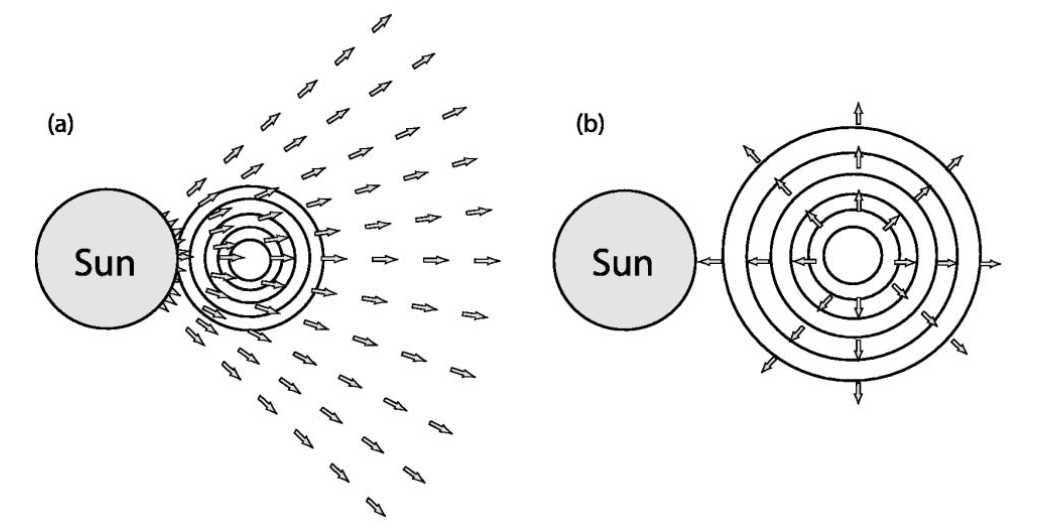
\includegraphics[width=0.9\linewidth]{imag/expansión.png}
    \caption[Evolución morfológica de la CME debida a efectos convectivos y gradientes de presión]{Efectos cinematicos en la evolución de la CME. En a) se muestra la evolución convectiva o expansión esférica; y en b) se muestra la expansión de la \ac{CME}\index{Coronal Mass Ejection} causada por un gradiente de presión entre ella y el viento solar ambiental, \cite{riley-2004}.}
    \label{fig:expansión}
\end{figure}

Entonces, al considerar ambas contribuciones en la expansión de la \ac{CME}\index{Coronal Mass Ejection} se puede llegar a encontrar algo similar a lo mostrado por la simulación MHD de \cite{odstrcil-2002}, la cual se muestra en la imagen \ref{fig:expansiónMHD}, en donde se puede ver como la \ac{CME}\index{Coronal Mass Ejection} presenta una deformación que la aplasta en la dirección de su propagación y la expande perpendicularmente a su dirección de propagación. Cabe señalar que esta simulación empieza con la estabilización de las condiciones del viento solar antes de producir la CME, por lo que se integran las ecucaciones del viento solar para cinco días (250 horas de la simulación) para luego producir la CME. Por lo que, el panel izquierdo de la figura \ref{fig:expansiónMHD} muestra la evolución de la \ac{CME}\index{Coronal Mass Ejection} 42 horas después de la generación de la misma.
\begin{figure}[H]
\centering
    \includegraphics[width=1\linewidth]{imag/expansión MHD.png}
    \caption[Resultados de velocidad, campo magnético y densidad del viento solar generados por la simulación hecha por \cite{odstrcil-2002}]{Propagación de una \ac{CME}\index{Coronal Mass Ejection} en la heliosfera, en donde la escala de colores muestra el mapa de velocidades, la densidad del plasma se muestra en relación a la densidad de líneas negras y el campo magnetico en relación a la densidad de líneas rojas. Se muestra la evolución de la \ac{CME}\index{Coronal Mass Ejection} en 4 tiempos: 292, 304, 320 y 350 horas después de empezar a correr la simulación}
    \label{fig:expansiónMHD}
\end{figure}

Por otro lado, las propiedades de las \acp{CME}\index{Coronal Mass Ejection} se pueden ver influenciadas por la interacción con el viento solar (SW) y con el campo magnético interplanetario (IMF), una primera consecuencia de esta interacción es la aceleración de \acp{CME}\index{Coronal Mass Ejection} lentas y la desaceleración de las \acp{CME}\index{Coronal Mass Ejection} rápidas para homogeneizar la velocidad en el viento solar, también cuando interactúan con estructuras corrotatorias del viento solar como nubes de viento rápido en las regiones de interacción corrotatoria (CIRs) o con otras CMEs.

La aceleración de propagación de las \acp{CME}\index{Coronal Mass Ejection} se ha estudiado de forma estadística, \cite[e.g.][]{gallagher-2003, zhang-2006} describen la cinemática de una \ac{CME}\index{Coronal Mass Ejection} a partir de observaciones de Transition Region and Coronal Explorer (TRACE), el Ultraviolet Coronagraph Spectrometer (UVCS) y el Large Angle and Spectroscopic Coronagraph (LASCO). Se encuentra que el perfil de la aceleración de una \ac{CME}\index{Coronal Mass Ejection} es como el mostrado en la gráfica \ref{fig:perfilaceleración}, en donde se presenta una etapa de \textbf{iniciación} con aceleración nula, luego una etapa de \textbf{aceleración} con una aceleración dependiente del tiempo, puesto que la velocidad no es lineal con respecto a la altura, seguida de una etapa de \textbf{propagación} en donde la aceleración se convierte en residual, ya que disminuye hasta generar una velocidad casi constante de propagación.

\begin{figure}[H]
\centering
    \includegraphics[width=0.9\linewidth]{imag/perfil de aceleración.png}
    \caption[Gráfica de velocidad de propagación de la CME en función del tiempo, con sus diferentes etapas]{Perfil de aceleración de una \ac{CME}\index{Coronal Mass Ejection} y de su Flare asociada, mostrados como sus velocidades en función del tiempo. Se muestran las tres fases de la dinámica de la \ac{CME}\index{Coronal Mass Ejection} y de la Flare, \cite{zhang-2006}.}
    \label{fig:perfilaceleración}
\end{figure}

Por ejemplo, en \cite{gallagher-2003} se estudia un evento de CME, tomando el del 21 de abril de 2002, generado en NOAA 9906 a las 00:43 UT, se observó su iniciación y propagación, tomando como punto de referencia su frente. Se generó los datos mostrados en las gráficas \ref{fig:ejemploperfilaceleración}.

\begin{figure}[H]
centering
    \includegraphics[width=0.9\linewidth]{imag/ejemploperfilaceleración.png}
    \caption[Gráficas experimentales de altura, velocidad de propagación y aceleración de la CME en función del tiempo]{Perfil de altura, velocidad y aceleración de la \ac{CME}\index{Coronal Mass Ejection} del 21 de abril de 2002 a las 00:43 UT, en función del tiempo. Así mismo, el flujo de rayos X debido a su Flare asociada, en función del tiempo. Los círculos rellenos son valores derivados de la gráfica de altura vs tiempo, los demás simbolos señalan las observaciones del TRACE, UVCS y del LASCO. La linea continua indica la curva con el mejor ajuste para los datos. \cite{gallagher-2003}.}
    \label{fig:ejemploperfilaceleración}
\end{figure}

En las gráficas \ref{fig:ejemploperfilaceleración} se muestra el perfil de velocidad esperado, \ref{fig:perfilaceleración}. Se puede identificar las fases de la dinámica de la CME, (inicial, aceleración y propagación) quedando en evidencia el comportamiento de la fase de propagación, en donde la aceleración se reduce y la velocidad se mantiene casi constante, por lo que la gráfica de altura vs tiempo tendrá un comportamiento casi lineal en el tiempo de la fase de propagación.

\section{Clasificación}
Una forma de clasificar las \acp{CME}\index{Coronal Mass Ejection} es a través de su lugar de origen en la superficie solar, así como del intervalo de tiempo que hay entre dos \acp{CME}\index{Coronal Mass Ejection} consecutivas por lo que se encuentran las erupciones simultaneas, homólogas y gemelas. Las \acp{CME}\index{Coronal Mass Ejection} simultaneas se considera a aquellas que ocurren en diferentes regiones activas del Sol pero aproximadamente al mismo tiempo, además de ello tienen propiedades similares, un estudio estadístico basado en datos de octubre de 1991 a diciembre de 1998 (\cite{Pevtsov_2000}) mostró que un tercio de todos las regiones activas (AR) presentan bucles transecuatoriales, independientemente del ciclo solar, lo que sugiere que las regiones activas de la superficie solar pueden estar inter-conectadas magnéticamente aunque se encuentren en hemisferios opuestos del Sol. Por lo que al estar inter-conectadas por bucles de campo magnético se puede presentar inestabilidades que se propaguen entre dichas regiones. 

Las \acp{CME}\index{Coronal Mass Ejection} homólogas se clasifican como las \acp{CME}\index{Coronal Mass Ejection} consecutivas que ocurren en unas misma región activa pero con una diferencia de tiempo que según \cite[~p.10]{lugaz-2017} es de al rededor de 15 horas, también menciona las \acp{CME}\index{Coronal Mass Ejection} cuasi-homologas las cuales tienen un intervalo de ocurrencia entre sí de 15 a 18 horas. Es más frecuente encontrar \acp{CME}\index{Coronal Mass Ejection} con poco tiempo de espera entre si indicando una alta relación pero en regiones diferentes, es decir el caso de las \acp{CME}\index{Coronal Mass Ejection} simultaneas, pero que si se concentra en una región activa (AR) la estadística muestra que es más frecuente encontrar \acp{CME}\index{Coronal Mass Ejection} con tiempos de espera más grandes. Entonces es más frecuente encontrar en la misma región activa \acp{CME}\index{Coronal Mass Ejection} con tiempos de espera grandes (al rededor de 30 horas) lo que clasificaría como \acp{CME}\index{Coronal Mass Ejection} "quiasi-homologous". Además, hay casos en los que se registraron \acp{CME}\index{Coronal Mass Ejection} gemelas, es decir que se produjeron en el mismo lugar, pero con minutos de diferencia, esto está relacionado con la eficiencia de la aceleración de partículas, \cite{lugaz-2017}.

Las \acp{CME}\index{Coronal Mass Ejection} gemelas ...


\section{Comportamiento en el medio interplanetario}
Las \acp{CME}\index{Coronal Mass Ejection} al salir al medio interplanetario generan una modificación drástica de las características del viento solar al arrastrar lineas de campo magnético a través de las superficies de Alfvén, éstas son superficies tridimensionales en donde la velocidad del flujo de plasma es igual a la velocidad de Alfvén.

Diferentes estudios han utilizado cuerdas de flujo, por ejemplo \cite{singh-2025} indica un modelo que se basa en una cuerda de flujo que se propaga desde el Sol, con dimensiones que dependen de la ubicación angular de las partes de la CME. Entonces, se mencionan las dimensiones de la cuerda de flujo y sus velocidades de propagación y expansión.
\begin{align}
    R(\phi)&=\frac{R_p}{R_t}r(\phi)\\
    r(\phi)&=R_t\cos^n\left(\frac{\pi}{2}\frac{\phi}{\phi_{hw}}\right)\\
    |\mathbf{V_{rad}}| &= V_{CME} \cdot \frac{1}{1+\frac{R_p}{R_t}}\\
    \mathbf{|V_{exp}(r_p)|} &= \mathbf{|V_{rad}|}{ \cdot \frac{r_p}{R_t}}
\end{align}
Donde $\phi$ es una coordenada toroidal, $R(\phi)$ es el radio de la sección transversal de la cuerda de flujo, $r(\phi)$ es la distancia desde el origen hasta la cuerda de flujo (otra coordenada toroidal), $n$ es un parámetro para ajustar la planitud de la forma de la cuerda de flujo y $\phi_{hw}$ es el angulo medio de la cuerda. Lo demás, $R_p$, $R_t$, $r_p$ y $V_{CME}$ son solamente parámetros ajustables.
Otro trabajo es el de \cite{mayank-2023}, en el que se utiliza un modelo que considera la interacción de una \ac{CME}\index{Coronal Mass Ejection} con el viento solar para luego y con otras CMEs. Este paper da información sobre las velocidades de las eyecciones de masa coronal (Coronal Mass Ejection, CME), su comportamiento a lo largo de su propagación y expansión en el medio interplanetario, además de considerar su interacción con el viento solar y desarrolla una simulación bajo diferentes técnicas de simulación usando el modelo SWASTi-CME. Menciona que los parámetros utilizados para simular el viento solar rápido son: $v_{fsw}=650\text{  km s}^{-1}$ para su velocidad, $n_{fsw}=200 \text{  cm}^{-3}$ su densidad, $B_{fsw}=300\text{  nT}$ su campo magnético. Además, menciona los parámetros utilizados para simular la \ac{CME}\index{Coronal Mass Ejection} emitida, una densidad $\rho_{CME}=10^{-18}\text{  kg m}^{-3}$, una temperatura de $T_{CME}=0.8\text{ MK}$, un flujo de campo magnético $\phi_{Mag}=10^{12}\text{ Wb}$.

El paper parte analizando las partes necesarias para la simulación, por lo que menciona la simulación del viento solar antes de la simulación de la CME. La primera la hace con ayuda de las ecuaciones de la magnetohidrodinámica, que son ecuaciones que vienen del principio de la conservación de la energía y del momentum. La segunda se hace con dos geometrías diferentes, una manera de simular una \ac{CME}\index{Coronal Mass Ejection} es a través de una geometría de cono elíptico con centro en el Sol con ecuaciones que modelan una \ac{CME}\index{Coronal Mass Ejection} propagándose a través del mismo, pero hay que tener en cuenta que este modelo funciona para distancias cercanas al Sol, otra manera de simular la \ac{CME}\index{Coronal Mass Ejection} es a través de una línea de flujo de campo magnético que es un loop que nace y muere en el Sol. Cabe señalar que el modelado de las \acp{CME}\index{Coronal Mass Ejection} contiene propiedades como la velocidad de expansión, velocidad de propagación, así como dirección.
Hay una parte en la que analiza el comportamiento de \acp{CME}\index{Coronal Mass Ejection} consecutivas que fueron simuladas con base en parámetros medidos experimentalmente en eventos específicos, por lo que muestra cómo sería el comportamiento de una segunda \ac{CME}\index{Coronal Mass Ejection} detrás de una primera \ac{CME}\index{Coronal Mass Ejection} que ocurrió antes.
También hace una comparación entre los datos dados por la simulación y los observados por naves espaciales reales, ya que gracias a una nave espacial virtual que recopila información dentro de la simulación se pueden cotejar lo observado con la simulación. Luego utiliza esta simulación para compararla con los datos recopilados in situ por naves espaciales, datos como la densidad del plasma, su velocidad radial, temperatura y campo magnético radial, mostrando que la concordancia entre lo simulado y lo observado es óptima.
También se encontró que la velocidad del viento solar influye en el comportamiento de la densidad de la CME; además, se menciona que la \ac{CME}\index{Coronal Mass Ejection} se estabilizará (llegará a su estado estacionario) más rápido entre más irregular sea el viento solar, por lo que considerar el viento solar en la simulación es fundamental.

Finalmente, el paper menciona que el frente de la \ac{CME}\index{Coronal Mass Ejection} puede enfrentarse a una fuerza de arrastre que bien puede ser negativa o positiva; la primera es debida a que la \ac{CME}\index{Coronal Mass Ejection} empuja el viento solar presente en su camino, la segunda es debida a una atracción por parte del viento solar sobre el frente de la CME, consecuencia de la diferencia de velocidades entre la \ac{CME}\index{Coronal Mass Ejection} y el viento solar, justificando esta fuerza de arrastre como el intercambio del momentum entre la \ac{CME}\index{Coronal Mass Ejection} y el viento solar. Por lo que, la fuerza de arrastre afecta la distribución de las propiedades de la CME, tales como su velocidad, su densidad, así como su tiempo de llegada a la Tierra, además de su morfología y dinámica.

\section{Detección y observación de CMEs}
La observación y estudio de estos fenómenos es gracias a mediciones in situ, observaciones remotas y a simulaciones numéricas.
Las \acp{CME}\index{Coronal Mass Ejection} observadas se han recopilado en catálogos de \acp{CME}\index{Coronal Mass Ejection} tales como el Coordinated Data Analysis Workshop (CDAW) o el Heliospheric Cataloguing, Analysis and Techniques Service (HELCATS).
El Generador de imágenes de eyecciones de masa coronal o Solar Mass Ejection Imager (SMEI) fue lanzado en 2003, siendo el primero de una nueva clase de instrumentos llamados Generadores de imágenes heliosféricas. El SMEI puede observar las diferentes etapas de evolución de una CME, desde su origen hasta su propagación a 1 AU.

SOLAR PROBE PLUS
SOHO con el intrumento CDS
HINODE con el instrumento EIS
SDO con el instrumento EVE

En \cite{mayank-2023}, se muestra, a través de una simulación usando el modelo SWASTi-CME, el comportamiento de una \ac{CME}\index{Coronal Mass Ejection} cuando interactúa con el viento solar, además de ver el impacto de las condiciones del viento solar en la propagación y evolución de la CME. Se describe el modelo SWASTi-CME como un modelo semi-empírico en 3D basado en física desarrollado para el estudio e investigación del clima espacial, es semi-empirico en un rango de 1 radio solar a los 21.5 radios solares, además de estar basado en MHD en el rango de 0.1AU a 2.1AU. Este modelo consta de dos representaciones de las CMEs, una es a través de un cono elíptico y el otro es a través de una linea de flujo. Primero se busca modelar el plasma del viento solar, por lo que se debe utilizar una velocidad ($V_{in}$) en la frontera, a 0.1AU, esta velocidad está dada por la versión modificada de la relación Wang-Sheeley-Arge.

\begin{equation}
V_{in}=\nu_{1}+\frac{\nu_{2}}{(1+f_{s})^{2/9}}\times \left( 1.0-0.8\exp\left( -\left( \frac{d}{w}\right)^{\beta} \right)\right)^{3}
\end{equation}

Donde $\nu_1$, $\nu_2$ y $\beta$ son parámetros independientes que se toman como 250 km/s, 675 km/s y 1.25, respectivamente. Además, $f_s$ es el factor de expansión del tubo de flujo y $d$ es la separación angular mínima del punto de pie del límite del agujero coronal, mientras que $w$ es la mediana del valor $d$para aquellas líneas de campo que alcanzan la ubicación de la Tierra.
Ahora, para la densidad inicial se tiene en cuenta la conservación de la energía a 0.1AU y la temperatura se obtiene de asumir una presión térmica constante. Así pues, en el paper \cite{mayank-2022}, se toma la densidad asociada al viento rápido como $n_{fsw}=200 cm^{-3}$, el campo magnético como $B_{fsw}=300nT$ y una presión térmica de 6.0 nPa en la frontera inicial. 

Ya para la simualción, \cite{mayank-2023}, utilizó las ecuaciones:
\[\frac{\partial \rho}{\partial t} + \nabla \cdot (\rho \mathbf{v}) = 0 \tag{4}\]

\[\frac{\partial \mathbf{m}}{\partial t} + \nabla \cdot \left[ \mathbf{mv} - \mathbf{BB} + \left( p + \frac{B^2}{2} \right) \mathbf{I} \right] = \rho \mathbf{g} \tag{5}\]

\[\frac{\partial \mathbf{B}}{\partial t} - \nabla \times (\mathbf{v} \times \mathbf{B}) = 0 \tag{6}\]

\[\frac{\partial E_t}{\partial t} + \nabla \cdot \left[ \left( \frac{\rho v^2}{2} + \frac{\gamma p}{\gamma - 1} \right) \mathbf{v} + \mathbf{B} \times (\mathbf{v} \times \mathbf{B}) \right] = \mathbf{m} \cdot \mathbf{g}, \tag{7}\]

donde $\rho$ es la densidad de masa, $\mathbf{v}$ es la velocidad, $\mathbf{m}$ es la densidad de momento ($\rho \mathbf{v}$), $\mathbf{B}$ es el campo magnético, $p$ es la presión térmica isotrópica, $\mathbf{g}$ es la aceleración gravitacional ($-\frac{GM_{\odot}}{r^2}$), $E_t$ es la densidad de energía total, y $\gamma (=5/3)$ es la relación de calores específicos del plasma del viento solar.

Ahora, \cite{mayank-2023} modela una \ac{CME}\index{Coronal Mass Ejection} utilizando dos geometrías, una es un cono elíptico con origen el el Sol y el otro es a través de una linea de flujo magnético. Para el  cono elíptico, se aproxima la forma de una \ac{CME}\index{Coronal Mass Ejection} como un tubo hueco que se expande, compuesto por dos conos truncados unidos por una sección central cilíndrica, luego se inserta una \ac{CME}\index{Coronal Mass Ejection} con esta forma y con una velocidad, una densidad  y una temperatura, a través de las siguientes ecuaciones:

 
 
\begin{equation}
\left( \frac{\phi-\phi_{{CME}}}{w(t)} \right)^{2}+\left( \frac{\theta-\theta_{CME}}{h(t)} \right)^{2}<1
\end{equation}

\begin{equation}
w(t)=\varphi_{hw}\cdot \sin\left[\frac{\pi}{2}\frac{(t-t_{\text{onset}})}{t_{half}} \right]
\end{equation}

\begin{equation}
h(t)=\varphi_{hh}\cdot \sin\left[\frac{\pi}{2}\frac{(t-t_{\text{onset}})}{t_{half}} \right]
\end{equation}

\begin{equation}
t_{half}=R_{in}\cdot \frac{\tan(\varphi_{hw})}{\nu_{CME}}
\end{equation}

 
Donde $\phi_{CME}$ y $\theta_{CME}$ son la longitud y latitud del centro de la CME, $w(t)$ y $h(t)$ son el ancho y la altura dependientes del tiempo de la CME, $\varphi_{hw}$ y $\varphi_{hh}$ son la mitad del ancho y la mitad de la altura angular del CME, $t_{onset}$ es el tiempo en el que inicia la inyección y $t_{half}$ es la mitad del tiempo de inserción del CME

Ya para una cuerda de flujo, se utiliza el modelo FRi3D para modelar la cuerda, la cual incorpora el campo magnético tridimensional relacionado a la CME. La geometria de la \ac{CME}\index{Coronal Mass Ejection} es como la de un croissantp. La variación del radio de la sección transversal de la \ac{CME}\index{Coronal Mass Ejection} se puede definir como :

\begin{equation}
R(\phi)=\frac{R_{t}}{R_{p}}\cdot r(\phi)
\end{equation}

\begin{equation}
R_{p}=R_{t}\cdot \tan(\varphi_{hh})
\end{equation}

\begin{equation}
r(\phi)=R_{t}\cdot \cos^{n}\left( \frac{\pi}{2} \frac{\phi}{\varphi_{{hw}}} \right)
\end{equation}


Donde $R_t$ es la distancia heliosferica al vertice del \ac{CME}\index{Coronal Mass Ejection} (distancia toroidal), $R_p$ es el radio de la sección transversal en el vértice (altura poloidal). Además, $r(\phi)$ es la distancia radial al eje de la \ac{CME}\index{Coronal Mass Ejection} desde el centro de los puntos de apoyo en la superficie solar.

Para el campo magnético dentro de la CME, o mejor dicho sus lineas de campo magnético, se utilizó la ecuación:
\begin{equation}
B=B_{axis}\cdot \exp{\left(\frac{-1}{2\sigma^{2}}\frac{R_{t}\cdot \vec{r}}{R_{p}\cdot r(\phi)}\right)}
\end{equation}

Donde $B_{axis}$ es la intensidad del campo magnético en el eje de la línea de flujo a un ángulo $\phi$ y $\sigma$ es el coeficiente de desviación estándar de la distribución. Con $R_t$ y $R_p$ las alturas toroidales y poloidales respectivamente, las cuales tiene una dependencia con el tiempo, a la vez de con una taza de expansión, así:
\begin{equation}
R_{t}(t)=R_{t}(0)+\nu_{t}\cdot t
\end{equation}

\begin{equation}
R_{p}(t)=R_{p}(0)+\nu_{p}\cdot t
\end{equation}

Donde $R_t(0)$ y $R_p(0)$ son los radios iniciales, toroidal y poloidal a 0.1 AU. Además, $\nu_t$ y $\nu_p$ son las velocidades a las que aumentan los radios, toroidal y poloidal. Por lo que la velocidad efectiva de la \ac{CME}\index{Coronal Mass Ejection} es la suma de estas dos velocidades.

Ahora bien, usando el modelo de cono elíptico, \cite{mayank-2023} compara resultados experimentales con resultados de la simualción, obteniendo lo que se muestra en la imagen \ref{fig:SWASTi-CME compa}.

\begin{figure}[H]
\centering
    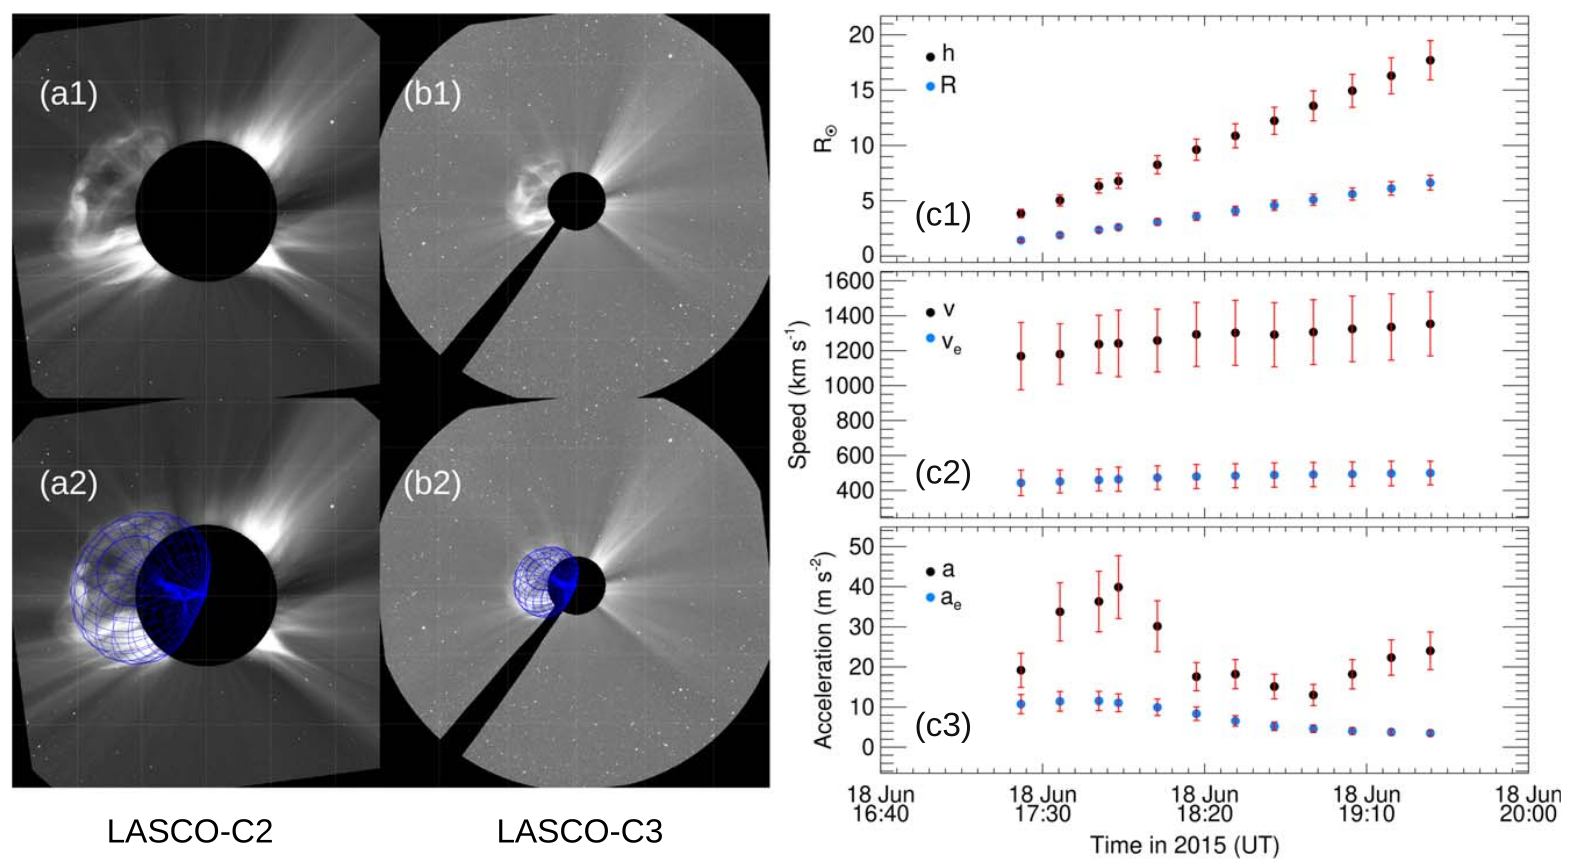
\includegraphics[width=1\linewidth]{imag/SWASTI_CME.png}
    \caption[Resultados del modelo usado en \cite{mayank-2023} sobre la cinemática de la CME, comparado con datos experimentales]{Imagenes de los coronografos LASCO-C2 (a1) y C3 (b1), del 18 de junio de 2015 en CR2165. Las imagenenes a2 y b2 presentan los resultados de utilizar el modelo de cono elíptico (en azul), sobre la misma imagen a1 y b1. En la parte derecha se muestra la evolución de la altura ($h$), velocidad ($V$) y aceleración ($a$) de la \ac{CME}\index{Coronal Mass Ejection} en función del tiempo (puntos negros), además del ancho ($R$), la velocidad de expansión ($v_e$) y la aceleración de expansión ($a_e$) en función del tiempo.}
    \label{fig:SWASTi-CME compa}
\end{figure}
De la imagen \ref{fig:SWASTi-CME compa} se puede ver que la velocidad de expansión ($V_e$) se mantiene al rededor de los $400 \text{km s}^{-1}$ durante toda la propagación, además se muestra que la aceleración de expansión disminuye una vez se haya superado la etapa de aceleración de la CME, es decir, dentro de la etapa de propagación (después del pico alcanzado por la aceleración de la CME).
Ahora bien, \cite{mayank-2023} también coloca una nave espacial virtual dentro de la simulación a una distancia de 1AU para recopilar datos y compararlos con los datos medidos experimentlamente in situ. Así pues, tomó una \ac{CME}\index{Coronal Mass Ejection} de CR2238 y la simuló para luego generar la comapración mostrada en la imagen \ref{ResultadoscomparadosSWASTI}, evidenciando que la evolución de una \ac{CME}\index{Coronal Mass Ejection} a una distancia de 1AU coincide en buena medida con los modelos utilizados.
\begin{figure}[H]
\centering
    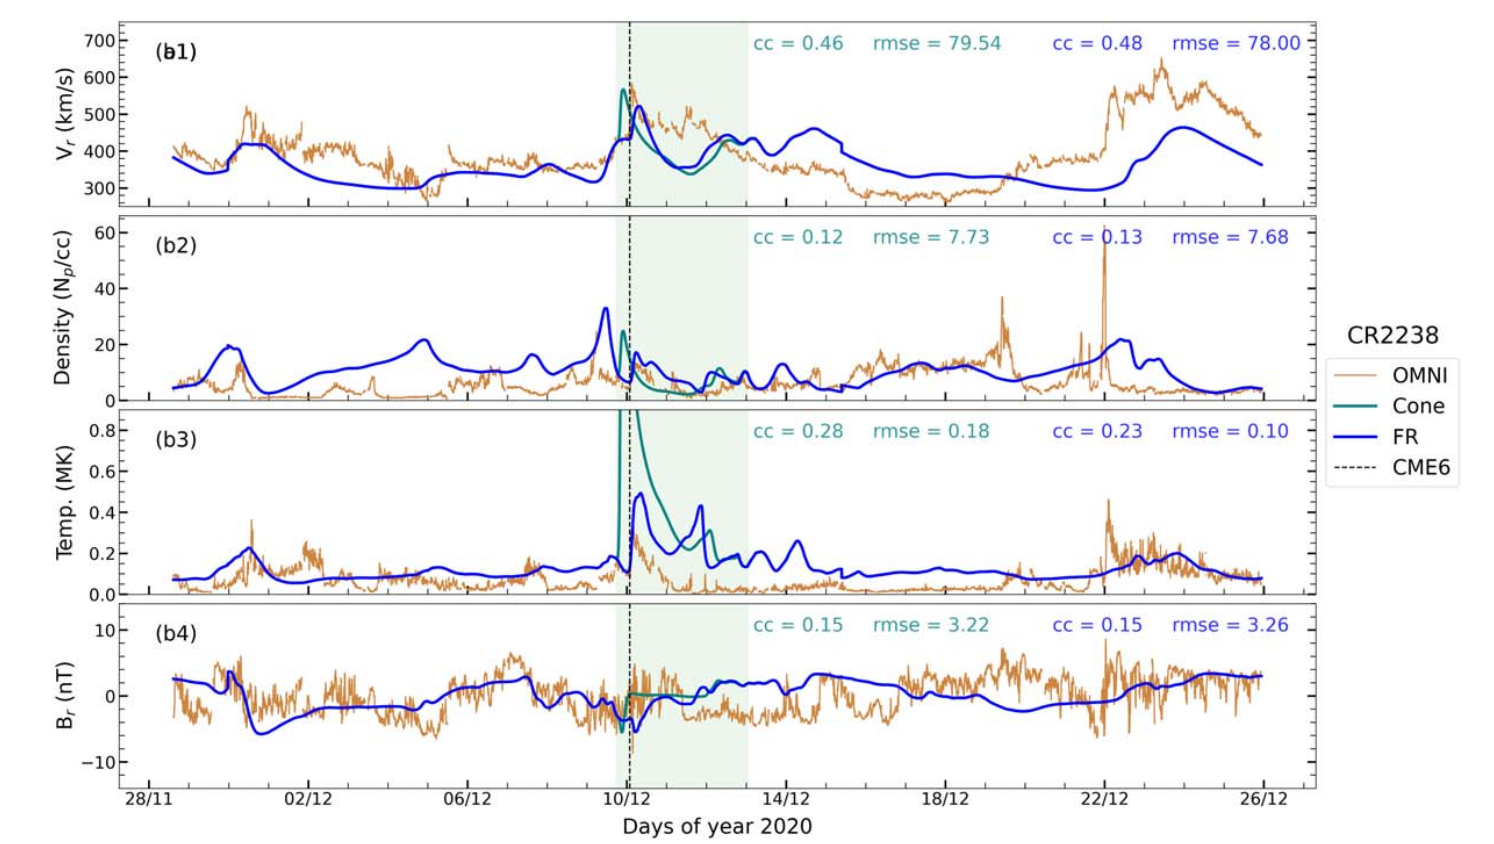
\includegraphics[width=1\linewidth]{imag/ResultadoscomparadosSWASTI.png}
    \caption[Gráficas de velocidad radial, densidad, temperatura y campo magnético radial tomados por OMNI comparados con la simualción de \cite{mayank-2023}]{Gráficas de velocidad radial ($V_R$), densidad, temperatura y campo magnético radial ($B_r$), tomados de OMNI (linea naranja) y de las simulaciones: Cono elíptico (linea verde) y Cuerda de flujo (linea azul). También, la línea punteada indica la llegada de la CME, que en el paper llaman CME6}
    \label{fig:ResultadoscomparadosSWASTI}
\end{figure}

Finalmente \cite{mayank-2023} señala que cuando un \ac{CME}\index{Coronal Mass Ejection} se propaga  expandiéndose en un medio no uniforme y denso su volumen resultante será menor en comparación al caso en el que se propaga en un medio menos denso o tenue, además de uniforme. Además, la no uniformidad del viento solar está relacionada con el tiempo en el que la \ac{CME}\index{Coronal Mass Ejection} alcanza su estabilidad, de tal forma que entre más irregular sea el viento solar, más rápido la \ac{CME}\index{Coronal Mass Ejection} llegará a su estado estacionario.

Por otro lado, el frente de la \ac{CME}\index{Coronal Mass Ejection} puede experimentar una fuerza de arrastre positiva o negativa, la primera es debida a que la \ac{CME}\index{Coronal Mass Ejection} empuja el viento solar presente en su camino y la segunda es debida a una atracción debida a las características del viento solar. Esta fuerza de arrastre es debida, en general, al intercambio de momentum entre las \acp{CME}\index{Coronal Mass Ejection} y el viento solar del medio.
Así pues, la fuerza de arrastre mostrada en \cite{mayank-2023} es de la forma:
\begin{equation}
F_{\text{arrastre}}=\frac{1}{2}C_{d}A\rho_{sw}|\nu_{CME}-\nu_{sw}|(\nu_{CME}-\nu_{sw})
\end{equation}

Donde $C_d$ es el coeficiente de arrastre adimensional y representa el nivel de interacción entre la \ac{CME}\index{Coronal Mass Ejection} y el medio, $A$ es el área que está en contacto con el frente de la \ac{CME}\index{Coronal Mass Ejection} y el viento solar, $\rho_{sw}$ es la densidad del viento solar ambiente, $\nu_{CME}$ es la velocidad de la \ac{CME}\index{Coronal Mass Ejection} así como $\nu_{sw}$ es la velocidad del viento solar. Cuando la fuerza de arrastre es positiva indica que el \ac{CME}\index{Coronal Mass Ejection} es el que está empujando el medio del viento solar, por otro lado, si la fuerza de arrastre es negativa indicaría que es el viento solar es el que está tirando de la CME, debido a sus diferencias de velocidad. Por lo que, la fuerza de arrastre afecta la distribución de las propiedades de la CME, tales como su velocidad, su densidad, entre otros, así como su tiempo de llegada a la Tierra, además de su morfología y dinámica.


Otro trabajo de simulación de interacción de \acp{CME}\index{Coronal Mass Ejection} fue realizado por \cite{lugaz-2017}, en donde simula la interacción de dos \acp{CME}\index{Coronal Mass Ejection} que en principio son idénticas, con velocidades iguales, por lo que si el \ac{CME}\index{Coronal Mass Ejection} secundario alcanza y sobre pasa al primer \ac{CME}\index{Coronal Mass Ejection} producido es solamente por la interacción con el medio, el cual brinda una desaceleración el primer \ac{CME}\index{Coronal Mass Ejection} y una aceleración al segundo debido al gradiente de presión que hay justo detrás del primer \ac{CME}\index{Coronal Mass Ejection} y al frente del segundo CME. Se estudia la propagación de un \ac{CME}\index{Coronal Mass Ejection} secundario a través del viento solar perturbado por el paso del primer CME.
Ahora bien, el estudio toma dos líneas de flujo magnético tridimensional idénticas y las posiciona en el mismo lugar, pero con una diferencia de tiempo de 10 horas, se emite la primera línea de flujo magnético y después de 10 horas se emite la segunda, todo esto con el fin de comparar el caso en el que se emite una línea de flujo cuando no hay una perturbación en el medio (como es el caso de la primera línea de flujo que se lanza) y el caso en el que sí hay una perturbación en el medio cuando pasa por él la línea de flujo magnético emitida (como es el caso de la segunda línea que se propaga a través de un medio perturbado por la primera línea emitida).
Ya en la discusión y en los resultados, se menciona que el segundo choque es fundamental para que la interacción evolucione hasta tener características similares a múltiples nubes magnéticas, aumentando la geoefectividad de las \acp{CME}\index{Coronal Mass Ejection} al interactuar con la magnetosfera terrestre, además permite la homogeneización de la velocidad junto con el choque inverso que desacelera la segunda nube magnética. Todo en conjunto permite ver a 1AU que las eyecciones complejas debidas a la interacción de las \ac{CME}\index{Coronal Mass Ejection} presentan velocidades homogéneas.
\section{Influencia en el clima espacial}
Las eyecciones de masa coronal afectan el clima espacial desde que se generan en la corona solar, pasando por el medio interplanetario hasta llegar a que su campo magnético interactúe con los campos magnéticos de los planetas así como con sus superficies. El paso de las \ac{CME}\index{Coronal Mass Ejection} simples (individuales) a una distancia de 1 AU  tarda al rededor de un día, lo que indica que las perturbaciones de campo magnético en $B_z$ que genera pueden durar varias horas. Mientras que el paso de \acp{CME}\index{Coronal Mass Ejection} que interactúan, tarda al rededor de 3 días en llegar a una distancia de 1 AU según \cite[e.g.,][]{lugaz-2017}, lo que indicaría que la magnetosfera se enfrentaría al fuerte viento solar que traen las \acp{CME}\index{Coronal Mass Ejection} durante más tiempo.

La interacción con la magnetósfera de los planetas produce auroras boreales que son un indicativo de las tormentas geomagnéticas que corresponden a una distorsión del campo magnético de un planeta debido a un gran ingreso de energía y partículas energéticas provenientes del medio interplanetario hacia su magnetósfera. La causa de las tormentas geomagnéticas son las \acp{CME}\index{Coronal Mass Ejection} y los eventos de SEPs provenientes de las Llamaradas solares, las cuales pueden llegar a inyectar 6$GW$ de potencia en la magnetosfera terrestre. La magnetosfera es la combinación de campo magnético y plasma influenciado por el clima espacial, es gracias a la magnetosfera interactuando con partículas energéticas del viento solar que se forman las auroras boreales. Además, las tormentas geomagnéticas más intensas son causadas por eyecciones de masa coronal y no por las llamaradas solares, según \cite[e.g,][]{2014swcm.book.....H}.

El flujo de campo magnético es de sur a norte, por lo que si una nube magnética con un flujo de campo magnético de norte a sur interactúa con la magnetósfera, se presentarán diferentes reconexiones magnéticas, lo que influiría en la cantidad de líneas de campo magnético abiertas lo que a su vez afectaría la producción de auroras boreales, ya que estas empezarían a ser visibles en regiones más cercanas al ecuador. Además, habría lineas de campo expuestas que facilitarían el ingreso de plasma a la atmósfera terrestre.


Estas tormentas magnéticas pueden ser caracterizadas por el parámetro Dst o Disturbance Storm Time (Dst), esta medida dada en nano-Teslas (nT) permite determinar la intensidad de una tormenta geomagnética a través de la intensidad de la corriente anular o Ring Current que es una corriente de partículas cargadas (iones y electrones) que circula en dirección oeste a una altura de entre 2 y 7 radios terrestres. La Ring Current es importante ya que esta corriente es energizada por las tormentas geomagnéticas y según el nivel al que se energice se pueden clasificar dichas tormentas en: Condiciones tranquilas o ambiente (0 a $-30$ nT), tormenta leve con poca actividad ($-30$ a $-50$ nT), tormenta moderada co posibles perturbaciones ($-50$ a $-100$ nT), tormenta intensa generando posibles daños a sistemas electrónicos ($<$ $-100$ nT) y tormenta severa o extrema con un riesgo alto en la integridad de la electrónica en la superficie terrestre ($<$ $-200$ nT) según \cite{nhess-2018-92}, para tener una idea, el evento Carrington en 1859 que fue el evento de tormenta geomagnética más intenso registrado en la historia, tuvo un rango de Dst de entre -1600nT a -850nT mencionado en \cite[e.g.,][]{2014swcm.book.....H}. Así pues, entre más negativa sea la medida del Dst mayor fue la tormenta geomagnética asociada y por ende mayor habrá sido la \ac{CME}\index{Coronal Mass Ejection} que generó dicha tormenta.

Además, \cite{lugaz-2005} encuentra que las dos nubes magnéticas evolucionan hasta llegar a una forma similar a múltiples nubes magnéticas, presentando dos regiones con un campo magnético intenso separadas por una región de alta temperatura. Además, se encuentra que la primera nube magnetice está comprimida y la segunda está sobre-expandida. Ahora el campo magnético de las diferentes nubes magnéticas presentan un cambio de polaridad a medida que las nubes se propagan a 1 AU.

Además, se tiene otro parámetro para medir la intensidad de las perturbaciones geomagnéticas es el índice Kp, el cual cuantifica las perturbaciones en el campo magnético terrestre causadas principalmente por el viento solar y las eyecciones de masa coronal. El Kp se refiere a la variabilidad geomagnética medida en intervalos de 3 horas, los rangos en los que clasifica las tormentas geomagnéticas son: Entre $0-1$ es muy tranquilo, $2-3$ es tranquilo, $4$ es activo, $5$ es una tormenta geomagnética menor, $6$ es una tormenta geomagnética moderada, $7$ es una tormenta geomagnética fuerte, $8$ es una tormenta geomagnética severa y $9$ es una tormenta geomagnética extrema, \cite{nhess-2018-92}.

Por otro lado, la interacción entre dos \acp{CME}\index{Coronal Mass Ejection} podría generar una tormenta geomagnética de doble inmersión que es aquella en la que el Disturbance Storm Time (Dts) muestra dos descensos pronunciados separados en el tiempo, es decir, que el gráfico del Dst tiene dos mínimos, lo que sugiere dos fases de intensificación.

Otro fenómeno que ocurre gracias a la interacción de \acp{CME}\index{Coronal Mass Ejection} es la generación de eventos SEPs por el choque magnetohidrodinámico, simulado por \cite{2004ApJ...616L.171S}, así pues, entre el 1$\%$ y el 2$\%$ de las \acp{CME}\index{Coronal Mass Ejection} se relacionan con los eventos SEPs, según \cite{lugaz-2005}.


%explicar que es una tormenta geomagnética, que es clima espacial, dar ejemplos de las diferentes categorías de las tormentas geomagnéticas. Hablar más del índice Kp.

